\documentclass{article}
\usepackage[utf8]{inputenc}
\usepackage{tikz}
\usepackage[legalpaper, landscape, margin=0.5in]{geometry}
\title{VSV-Visualization}
\date{}
\begin{document}
\maketitle
\begin{figure}[h!]
\centering
\begin{tikzpicture}[draw=black, scale=0.75, transform shape]

\node[align=left] at (-0.5,5) {P0};
\draw [thick] (0.00000,5) -- (2.33161,5);
\node[align=center, above] at (1.16581,5) {$ins(2)$};% x_offset = 33.70293

\node[align=left] at (-0.5,4) {P1};

\node[align=left] at (-0.5,3) {P2};

\node[align=left] at (-0.5,2) {P3};

\node[align=left] at (-0.5,1) {P4};
\end{tikzpicture}
\caption{Concurrent History}
\end{figure}
\begin{figure}[h!]
\centering
\begin{tikzpicture}[draw=black, scale=0.75, transform shape]

\node[align=left] at (-0.5,5) {P0};
\draw [thick] (0.00000,5) -- (2.24524,5);
\node[align=center, above] at (1.12262,5) {$ins(10)$};% x_offset = 496.89291
\draw [thick] (38.25473,5) -- (39.73056,5);
\node[align=center, above] at (38.99222,5) {$ins(7)$};% x_offset = 496.89291

\node[align=left] at (-0.5,4) {P1};

\node[align=left] at (-0.5,3) {P2};

\node[align=left] at (-0.5,2) {P3};

\node[align=left] at (-0.5,1) {P4};
\end{tikzpicture}
\caption{Concurrent History}
\end{figure}
\begin{figure}[h!]
\centering
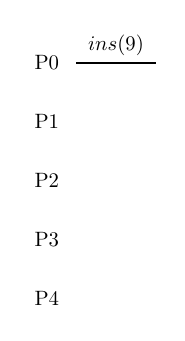
\begin{tikzpicture}[draw=black, scale=0.75, transform shape]

\node[align=left] at (-0.5,5) {P0};
\draw [thick] (0.00000,5) -- (1.34283,5);
\node[align=center, above] at (0.67102,5) {$ins(9)$};% x_offset = 568.85059

\node[align=left] at (-0.5,4) {P1};

\node[align=left] at (-0.5,3) {P2};

\node[align=left] at (-0.5,2) {P3};

\node[align=left] at (-0.5,1) {P4};
\end{tikzpicture}
\caption{Concurrent History}
\end{figure}
\begin{figure}[h!]
\centering
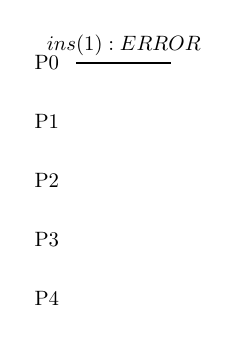
\begin{tikzpicture}[draw=black, scale=0.75, transform shape]

\node[align=left] at (-0.5,5) {P0};
\draw [thick] (0.00000,5) -- (1.60449,5);
\node[align=center, above] at (0.80225,5) {$ins(1):ERROR$};% x_offset = 709.71155

\node[align=left] at (-0.5,4) {P1};

\node[align=left] at (-0.5,3) {P2};

\node[align=left] at (-0.5,2) {P3};

\node[align=left] at (-0.5,1) {P4};
\end{tikzpicture}
\caption{Concurrent History}
\end{figure}
\begin{figure}[h!]
\centering
\begin{tikzpicture}[draw=black, scale=0.75, transform shape]

\node[align=left] at (-0.5,5) {P0};

\node[align=left] at (-0.5,4) {P1};
\draw [thick] (0.00000,4) -- (5.00952,4);
\node[align=center, above] at (2.50427,4) {$rem(1):ERROR$};% x_offset = 1157.71765

\node[align=left] at (-0.5,3) {P2};

\node[align=left] at (-0.5,2) {P3};

\node[align=left] at (-0.5,1) {P4};
\end{tikzpicture}
\caption{Concurrent History}
\end{figure}
\begin{figure}[h!]
\centering
\begin{tikzpicture}[draw=black, scale=0.75, transform shape]

\node[align=left] at (-0.5,5) {P0};

\node[align=left] at (-0.5,4) {P1};
\draw [thick] (0.00000,4) -- (3.19080,4);
\node[align=center, above] at (1.59497,4) {$ins(4)$};% x_offset = 1235.07690

\node[align=left] at (-0.5,3) {P2};

\node[align=left] at (-0.5,2) {P3};

\node[align=left] at (-0.5,1) {P4};
\end{tikzpicture}
\caption{Concurrent History}
\end{figure}
\begin{figure}[h!]
\centering
\begin{tikzpicture}[draw=black, scale=0.75, transform shape]

\node[align=left] at (-0.5,5) {P0};

\node[align=left] at (-0.5,4) {P1};

\node[align=left] at (-0.5,3) {P2};
\draw [thick] (0.00000,3) -- (2.61572,3);
\node[align=center, above] at (1.30750,3) {$rem(7)$};% x_offset = 1613.81775
\draw [thick] (11.54834,3) -- (12.65637,3);
\node[align=center, above] at (12.10193,3) {$rem(4)$};% x_offset = 1613.81775

\node[align=left] at (-0.5,2) {P3};

\node[align=left] at (-0.5,1) {P4};
\end{tikzpicture}
\caption{Concurrent History}
\end{figure}
\begin{figure}[h!]
\centering
\begin{tikzpicture}[draw=black, scale=0.75, transform shape]

\node[align=left] at (-0.5,5) {P0};

\node[align=left] at (-0.5,4) {P1};

\node[align=left] at (-0.5,3) {P2};
\draw [thick] (0.00000,3) -- (1.60791,3);
\node[align=center, above] at (0.80396,3) {$ins(5)$};% x_offset = 1728.65979
\draw [thick] (11.01379,3) -- (12.78845,3);
\node[align=center, above] at (11.90063,3) {$rem(6):ERROR$};% x_offset = 1728.65979

\node[align=left] at (-0.5,2) {P3};

\node[align=left] at (-0.5,1) {P4};
\end{tikzpicture}
\caption{Concurrent History}
\end{figure}
\begin{figure}[h!]
\centering
\begin{tikzpicture}[draw=black, scale=0.75, transform shape]

\node[align=left] at (-0.5,5) {P0};

\node[align=left] at (-0.5,4) {P1};

\node[align=left] at (-0.5,3) {P2};
\draw [thick] (0.00000,3) -- (1.60364,3);
\node[align=center, above] at (0.80139,3) {$ins(7)$};% x_offset = 1832.01721
\draw [thick] (10.89209,3) -- (12.35242,3);
\node[align=center, above] at (11.62183,3) {$rem(9)$};% x_offset = 1832.01721

\node[align=left] at (-0.5,2) {P3};

\node[align=left] at (-0.5,1) {P4};
\end{tikzpicture}
\caption{Concurrent History}
\end{figure}
\begin{figure}[h!]
\centering
\begin{tikzpicture}[draw=black, scale=0.75, transform shape]

\node[align=left] at (-0.5,5) {P0};

\node[align=left] at (-0.5,4) {P1};

\node[align=left] at (-0.5,3) {P2};
\draw [thick] (0.00000,3) -- (0.50000,3);
\node[align=center, above] at (0.24951,3) {$ins(1):ERROR$};% x_offset = 2329.90845
\draw [thick] (9.91968,3) -- (11.18823,3);
\node[align=center, above] at (10.55347,3) {$rem(5)$};% x_offset = 2329.90845

\node[align=left] at (-0.5,2) {P3};

\node[align=left] at (-0.5,1) {P4};
\end{tikzpicture}
\caption{Concurrent History}
\end{figure}
\begin{figure}[h!]
\centering
\begin{tikzpicture}[draw=black, scale=0.75, transform shape]

\node[align=left] at (-0.5,5) {P0};

\node[align=left] at (-0.5,4) {P1};

\node[align=left] at (-0.5,3) {P2};
\draw [thick] (0.00000,3) -- (2.18555,3);
\node[align=center, above] at (1.09229,3) {$rem(6):ERROR$};% x_offset = 2376.76953
\draw [thick] (26.33325,3) -- (28.32715,3);
\node[align=center, above] at (27.32983,3) {$rem(10)$};% x_offset = 2376.76953

\node[align=left] at (-0.5,2) {P3};

\node[align=left] at (-0.5,1) {P4};
\end{tikzpicture}
\caption{Concurrent History}
\end{figure}
\begin{figure}[h!]
\centering
\begin{tikzpicture}[draw=black, scale=0.75, transform shape]

\node[align=left] at (-0.5,5) {P0};

\node[align=left] at (-0.5,4) {P1};

\node[align=left] at (-0.5,3) {P2};
\draw [thick] (0.00000,3) -- (0.88525,3);
\node[align=center, above] at (0.44214,3) {$ins(5)$};% x_offset = 2509.75293
\draw [thick] (9.61499,3) -- (10.57617,3);
\node[align=center, above] at (10.09497,3) {$rem(7)$};% x_offset = 2509.75293

\node[align=left] at (-0.5,2) {P3};

\node[align=left] at (-0.5,1) {P4};
\end{tikzpicture}
\caption{Concurrent History}
\end{figure}
\begin{figure}[h!]
\centering
\begin{tikzpicture}[draw=black, scale=0.75, transform shape]

\node[align=left] at (-0.5,5) {P0};

\node[align=left] at (-0.5,4) {P1};

\node[align=left] at (-0.5,3) {P2};
\draw [thick] (0.00000,3) -- (1.08374,3);
\node[align=center, above] at (0.54150,3) {$ins(6):ERROR$};% x_offset = 2607.86523
\draw [thick] (10.32983,3) -- (11.68921,3);
\node[align=center, above] at (11.00952,3) {$ins(8)$};% x_offset = 2607.86523

\node[align=left] at (-0.5,2) {P3};

\node[align=left] at (-0.5,1) {P4};
\end{tikzpicture}
\caption{Concurrent History}
\end{figure}
\begin{figure}[h!]
\centering
\begin{tikzpicture}[draw=black, scale=0.75, transform shape]

\node[align=left] at (-0.5,5) {P0};

\node[align=left] at (-0.5,4) {P1};

\node[align=left] at (-0.5,3) {P2};

\node[align=left] at (-0.5,2) {P3};

\node[align=left] at (-0.5,1) {P4};
\draw [thick] (0.00000,1) -- (1.35840,1);
\node[align=center, above] at (0.67896,1) {$ins(4)$};% x_offset = 2706.48779
\draw [thick] (10.52612,1) -- (12.02954,1);
\node[align=center, above] at (11.27734,1) {$rem(1):ERROR$};% x_offset = 2706.48779
\end{tikzpicture}
\caption{Concurrent History}
\end{figure}
\begin{figure}[h!]
\centering
\begin{tikzpicture}[draw=black, scale=0.75, transform shape]

\node[align=left] at (-0.5,5) {P0};

\node[align=left] at (-0.5,4) {P1};

\node[align=left] at (-0.5,3) {P2};
\draw [thick] (0.00000,3) -- (1.08301,3);
\node[align=center, above] at (0.54150,3) {$rem(5)$};% x_offset = 2858.34888
\draw [thick] (11.62012,3) -- (12.53198,3);
\node[align=center, above] at (12.07593,3) {$ins(10)$};% x_offset = 2858.34888

\node[align=left] at (-0.5,2) {P3};

\node[align=left] at (-0.5,1) {P4};
\end{tikzpicture}
\caption{Concurrent History}
\end{figure}
\begin{figure}[h!]
\centering
\begin{tikzpicture}[draw=black, scale=0.75, transform shape]

\node[align=left] at (-0.5,5) {P0};

\node[align=left] at (-0.5,4) {P1};

\node[align=left] at (-0.5,3) {P2};
\draw [thick] (0.00000,3) -- (1.12354,3);
\node[align=center, above] at (0.56128,3) {$rem(10)$};% x_offset = 2908.77808
\draw [thick] (36.34106,3) -- (37.45410,3);
\node[align=center, above] at (36.89722,3) {$ins(5)$};% x_offset = 2908.77808

\node[align=left] at (-0.5,2) {P3};

\node[align=left] at (-0.5,1) {P4};
\end{tikzpicture}
\caption{Concurrent History}
\end{figure}
\begin{figure}[h!]
\centering
\begin{tikzpicture}[draw=black, scale=0.75, transform shape]

\node[align=left] at (-0.5,5) {P0};

\node[align=left] at (-0.5,4) {P1};

\node[align=left] at (-0.5,3) {P2};
\draw [thick] (0.00000,3) -- (1.31958,3);
\node[align=center, above] at (0.65967,3) {$rem(1):ERROR$};% x_offset = 2979.62866
\draw [thick] (35.90942,3) -- (37.57178,3);
\node[align=center, above] at (36.73999,3) {$rem(3):ERROR$};% x_offset = 2979.62866

\node[align=left] at (-0.5,2) {P3};

\node[align=left] at (-0.5,1) {P4};
\end{tikzpicture}
\caption{Concurrent History}
\end{figure}
\begin{figure}[h!]
\centering
\begin{tikzpicture}[draw=black, scale=0.75, transform shape]

\node[align=left] at (-0.5,5) {P0};

\node[align=left] at (-0.5,4) {P1};

\node[align=left] at (-0.5,3) {P2};

\node[align=left] at (-0.5,2) {P3};
\draw [thick] (0.00000,2) -- (2.65015,2);
\node[align=center, above] at (1.32471,2) {$ins(9)$};% x_offset = 3139.14941
\draw [thick] (11.28589,2) -- (13.00781,2);
\node[align=center, above] at (12.14673,2) {$rem(4)$};% x_offset = 3139.14941

\node[align=left] at (-0.5,1) {P4};
\end{tikzpicture}
\caption{Concurrent History}
\end{figure}
\end{document}
